
\section{第一部分}
%垂直居中
\begin{frame}
  \begin{center}
  需要居中的内容!
  \end{center}
\end{frame}

\begin{frame}
  \centering
  一些内容
\end{frame}

%幻灯片标题的使用
\begin{frame}
  \frametitle{第一部分第一张幻灯}
    一些内容
  \end{frame}

%项目编号的使用
\begin{frame}
  \frametitle{条目}
  \begin{itemize}
  \item 项目1
  \item 项目2
  \item 项目3
  \item 项目4
    \begin{itemize}
    \item 二级项目1
    \item 二级项目2
    \end{itemize}
  \end{itemize}
\end{frame}

%表格的使用
\begin{frame}
  \frametitle{表格}
  \begin{table}[htbp!]
    \centering
    \caption{主流机器学习框架}
    \begin{tabular}{c|c|c|c|c}
      \toprule[1pt]
      机器学习库	& 机构 & 支持语言  & 平台 & Tensor \\
      \toprule[1pt]
      TensorFlow	& Google & C++,Python &跨平台 & Good \\
 	  \hline
      Pytorch	&  Facebook& Python & 跨平台 & Good \\
 	  \bottomrule[1pt]
    \end{tabular}
  \end{table}
\end{frame}

% \begin{frame}
%   \rowcolors{2}{craneorange!25}{craneorange!50}
%   \begin{tabular}{r|r|r}
%   % \rowcolor{craneorange} 直角边  & 直角边  & 斜边 \\
%   机器学习库	& 机构 & 支持语言  \\
%   % 机器学习库	& 机构 & 支持语言  \\
%   % 机器学习库	& 机构 & 支持语言  \\
%   % $3$ & $4$ & $5$ \\
%   % 5 & 12 & 13 \\
%   % 7 & 24 & 25 \\
%   % 8 & 15 & 17 \\
%   \end{tabular}
% \end{frame}

\section{第二部分}

%区块的使用
\begin{frame}
  \frametitle{分析}
  \begin{block}{XXX 算法}
	\begin{itemize}
		\item 步骤1
	 	\item 步骤2
	 	\item 步骤3
	 \end{itemize}
  \end{block}
\end{frame}

%使用区块来强调内容
\begin{frame}
  \frametitle{强调}
  \begin{itemize}
  \item 这是内容
  \end{itemize}
  \only<1>\begin{block}{}
    这里蹦出来一个强调!
  \end{block}
\end{frame}




\section{第三部分}
%section中目录的使用
\begin{frame}
  \frametitle{技术影响力}
    \tableofcontents[currentsection,hideallsubsections]
\end{frame}

%插入图片
\begin{frame}
  \begin{figure}[!h]
    \centering
    % Requires \usepackage{graphicx}
    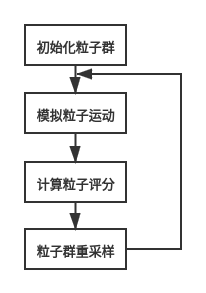
\includegraphics[width=2cm]{pics/mcl.png}\\
    \caption{logo图片样例}\label{pic6}
  \end{figure}
  \end{frame}

  %分栏实现图文混排
\begin{frame}
  分栏前面的一些内容!!
  \begin{columns}%0.6 0.4表示相对比例
  \column{0.6\textwidth}%<1->
  分栏的左侧,文字叙述。
  \column{0.4\textwidth}%<1->
  分栏的右侧插入了图片。
   \begin{figure}[!h]
    \centering
    % Requires \usepackage{graphicx}
    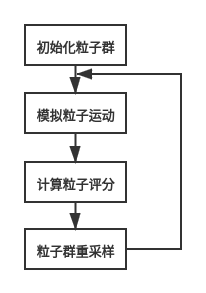
\includegraphics[width=4cm]{pics/mcl}\\
    \caption{logo图片样例}\label{pic6}
  \end{figure}
  \end{columns}
  分栏后面的一些内容!!
  \end{frame}

  \begin{frame}{Math} %数学公式
    \begin{equation*}
      e = \lim_{n\to \infty} \left(1 + \frac{1}{n}\right)^n
    \end{equation*}
  \end{frame}

  \begin{frame}
    \begin{block}{勾股定理}
    直角三角形的斜边的平方等于两直角边的平方和。
    可以用符号语言表述为:设直角三角形ABC,其中$\angle C=90^\circ$则有
    \begin{equation}
    AB^2=BC^2+AC^2
    \end{equation}
    \end{block}
    \end{frame}

